\documentclass[]{book}
\usepackage{lmodern}
\usepackage{amssymb,amsmath}
\usepackage{ifxetex,ifluatex}
\usepackage{fixltx2e} % provides \textsubscript
\ifnum 0\ifxetex 1\fi\ifluatex 1\fi=0 % if pdftex
  \usepackage[T1]{fontenc}
  \usepackage[utf8]{inputenc}
\else % if luatex or xelatex
  \ifxetex
    \usepackage{mathspec}
  \else
    \usepackage{fontspec}
  \fi
  \defaultfontfeatures{Ligatures=TeX,Scale=MatchLowercase}
\fi
% use upquote if available, for straight quotes in verbatim environments
\IfFileExists{upquote.sty}{\usepackage{upquote}}{}
% use microtype if available
\IfFileExists{microtype.sty}{%
\usepackage{microtype}
\UseMicrotypeSet[protrusion]{basicmath} % disable protrusion for tt fonts
}{}
\usepackage[margin=1in]{geometry}
\usepackage{hyperref}
\hypersetup{unicode=true,
            pdftitle={Statistical Tools for Causal Inference},
            pdfauthor={The SKY Community},
            pdfborder={0 0 0},
            breaklinks=true}
\urlstyle{same}  % don't use monospace font for urls
\usepackage{color}
\usepackage{fancyvrb}
\newcommand{\VerbBar}{|}
\newcommand{\VERB}{\Verb[commandchars=\\\{\}]}
\DefineVerbatimEnvironment{Highlighting}{Verbatim}{commandchars=\\\{\}}
% Add ',fontsize=\small' for more characters per line
\usepackage{framed}
\definecolor{shadecolor}{RGB}{248,248,248}
\newenvironment{Shaded}{\begin{snugshade}}{\end{snugshade}}
\newcommand{\KeywordTok}[1]{\textcolor[rgb]{0.13,0.29,0.53}{\textbf{#1}}}
\newcommand{\DataTypeTok}[1]{\textcolor[rgb]{0.13,0.29,0.53}{#1}}
\newcommand{\DecValTok}[1]{\textcolor[rgb]{0.00,0.00,0.81}{#1}}
\newcommand{\BaseNTok}[1]{\textcolor[rgb]{0.00,0.00,0.81}{#1}}
\newcommand{\FloatTok}[1]{\textcolor[rgb]{0.00,0.00,0.81}{#1}}
\newcommand{\ConstantTok}[1]{\textcolor[rgb]{0.00,0.00,0.00}{#1}}
\newcommand{\CharTok}[1]{\textcolor[rgb]{0.31,0.60,0.02}{#1}}
\newcommand{\SpecialCharTok}[1]{\textcolor[rgb]{0.00,0.00,0.00}{#1}}
\newcommand{\StringTok}[1]{\textcolor[rgb]{0.31,0.60,0.02}{#1}}
\newcommand{\VerbatimStringTok}[1]{\textcolor[rgb]{0.31,0.60,0.02}{#1}}
\newcommand{\SpecialStringTok}[1]{\textcolor[rgb]{0.31,0.60,0.02}{#1}}
\newcommand{\ImportTok}[1]{#1}
\newcommand{\CommentTok}[1]{\textcolor[rgb]{0.56,0.35,0.01}{\textit{#1}}}
\newcommand{\DocumentationTok}[1]{\textcolor[rgb]{0.56,0.35,0.01}{\textbf{\textit{#1}}}}
\newcommand{\AnnotationTok}[1]{\textcolor[rgb]{0.56,0.35,0.01}{\textbf{\textit{#1}}}}
\newcommand{\CommentVarTok}[1]{\textcolor[rgb]{0.56,0.35,0.01}{\textbf{\textit{#1}}}}
\newcommand{\OtherTok}[1]{\textcolor[rgb]{0.56,0.35,0.01}{#1}}
\newcommand{\FunctionTok}[1]{\textcolor[rgb]{0.00,0.00,0.00}{#1}}
\newcommand{\VariableTok}[1]{\textcolor[rgb]{0.00,0.00,0.00}{#1}}
\newcommand{\ControlFlowTok}[1]{\textcolor[rgb]{0.13,0.29,0.53}{\textbf{#1}}}
\newcommand{\OperatorTok}[1]{\textcolor[rgb]{0.81,0.36,0.00}{\textbf{#1}}}
\newcommand{\BuiltInTok}[1]{#1}
\newcommand{\ExtensionTok}[1]{#1}
\newcommand{\PreprocessorTok}[1]{\textcolor[rgb]{0.56,0.35,0.01}{\textit{#1}}}
\newcommand{\AttributeTok}[1]{\textcolor[rgb]{0.77,0.63,0.00}{#1}}
\newcommand{\RegionMarkerTok}[1]{#1}
\newcommand{\InformationTok}[1]{\textcolor[rgb]{0.56,0.35,0.01}{\textbf{\textit{#1}}}}
\newcommand{\WarningTok}[1]{\textcolor[rgb]{0.56,0.35,0.01}{\textbf{\textit{#1}}}}
\newcommand{\AlertTok}[1]{\textcolor[rgb]{0.94,0.16,0.16}{#1}}
\newcommand{\ErrorTok}[1]{\textcolor[rgb]{0.64,0.00,0.00}{\textbf{#1}}}
\newcommand{\NormalTok}[1]{#1}
\usepackage{longtable,booktabs}
\usepackage{graphicx,grffile}
\makeatletter
\def\maxwidth{\ifdim\Gin@nat@width>\linewidth\linewidth\else\Gin@nat@width\fi}
\def\maxheight{\ifdim\Gin@nat@height>\textheight\textheight\else\Gin@nat@height\fi}
\makeatother
% Scale images if necessary, so that they will not overflow the page
% margins by default, and it is still possible to overwrite the defaults
% using explicit options in \includegraphics[width, height, ...]{}
\setkeys{Gin}{width=\maxwidth,height=\maxheight,keepaspectratio}
\IfFileExists{parskip.sty}{%
\usepackage{parskip}
}{% else
\setlength{\parindent}{0pt}
\setlength{\parskip}{6pt plus 2pt minus 1pt}
}
\setlength{\emergencystretch}{3em}  % prevent overfull lines
\providecommand{\tightlist}{%
  \setlength{\itemsep}{0pt}\setlength{\parskip}{0pt}}
\setcounter{secnumdepth}{5}
% Redefines (sub)paragraphs to behave more like sections
\ifx\paragraph\undefined\else
\let\oldparagraph\paragraph
\renewcommand{\paragraph}[1]{\oldparagraph{#1}\mbox{}}
\fi
\ifx\subparagraph\undefined\else
\let\oldsubparagraph\subparagraph
\renewcommand{\subparagraph}[1]{\oldsubparagraph{#1}\mbox{}}
\fi

%%% Use protect on footnotes to avoid problems with footnotes in titles
\let\rmarkdownfootnote\footnote%
\def\footnote{\protect\rmarkdownfootnote}

%%% Change title format to be more compact
\usepackage{titling}

% Create subtitle command for use in maketitle
\newcommand{\subtitle}[1]{
  \posttitle{
    \begin{center}\large#1\end{center}
    }
}

\setlength{\droptitle}{-2em}
  \title{Statistical Tools for Causal Inference}
  \pretitle{\vspace{\droptitle}\centering\huge}
  \posttitle{\par}
  \author{The SKY Community}
  \preauthor{\centering\large\emph}
  \postauthor{\par}
  \predate{\centering\large\emph}
  \postdate{\par}
  \date{2019-04-13}

\usepackage{dsfont}
\newcommand{\uns}[1]{\mathds{1}[ #1 ]}
\usepackage{subfig}

\usepackage{amsthm}
\newtheorem{theorem}{Theorem}[chapter]
\newtheorem{lemma}{Lemma}[chapter]
\theoremstyle{definition}
\newtheorem{definition}{Definition}[chapter]
\newtheorem{corollary}{Corollary}[chapter]
\newtheorem{proposition}{Proposition}[chapter]
\theoremstyle{definition}
\newtheorem{example}{Example}[chapter]
\theoremstyle{definition}
\newtheorem{exercise}{Exercise}[chapter]
\theoremstyle{remark}
\newtheorem*{remark}{Remark}
\newtheorem*{solution}{Solution}
\let\BeginKnitrBlock\begin \let\EndKnitrBlock\end
\begin{document}
\maketitle

{
\setcounter{tocdepth}{1}
\tableofcontents
}
\chapter*{Introduction}\label{introduction}
\addcontentsline{toc}{chapter}{Introduction}

Tools of causal inference are the basic statistical building block
behind most scientific results. It is thus extremely useful to have an
open source collectively aggreed upon resource presenting and assessing
them, as well as listing the current unresolved issues. The content of
this book covers the basic theoretical knowledge and technical skills
required for implementing staistical methods of causal inference. This
means:

\begin{itemize}
\tightlist
\item
  Understanding of the basic language to encode causality,
\item
  Knowledge of the fundamental problems of inference and the biases of
  intuitive estimators,
\item
  Understanding of how econometric methods recover treatment effects,
\item
  Ability to compute these estimators along with an estimate of their
  precision using the statistical software R combined with latex using
  Rmarkdown.
\end{itemize}

All the notions and estimators are introduced using a numerical example
and simulations.

All the code behind this book is written in Rmarkdown and is publically
available on GitHub. Feel free to propose corrections and updates.

\part{The Two Fundamental Problems of
Inference}\label{part-the-two-fundamental-problems-of-inference}

When trying to estimate the effect of a program on an outcome, we face
two very important and difficult problems: \href{FPCI.html}{the
Fundamental Problem of Causal Inference (FPCI)} and \href{FPSI.html}{the
Fundamental Problem of Statistical Inference (FPSI)}.

In its most basic form, the FPCI states that our causal parameter of
interest (\(TT\), short for Treatment on the Treated, that we will
define shortly) is fundamentally unobservable, even when the sample size
is infinite. The main reason for that is that one component of \(TT\),
the outcome of the treated had they not received the program, remains
unobservable. We call this outcome a counterfactual outcome. The FPCI is
a very dispiriting result, and is actually the basis for all of the
statistical methods of causal inference. All of these methods try to
find ways to estimate the counterfactual by using observable quantities
that hopefully approximate it as well as possible. Most people,
including us but also policymakers, generally rely on intuitive
quantities in order to generate the counterfactual (the individuals
without the program or the individuals before the program was
implemented). Unfortunately, these approximations are generally very
crude, and the resulting estimators of \(TT\) are generally biased,
sometimes severely.

The Fundamental Problem of Statistical Inference (FPSI) states that,
even if we have an estimator \(E\) that identifies \(TT\) in the
population, we cannot observe \(E\) because we only have access to a
finite sample of the population. The only thing that we can form from
the sample is a sample equivalent \(\hat{E}\) to the population quantity
\(E\), and \(\hat{E}\neq E\). Why is \(\hat{E}\neq E\)? Because a finite
sample is never perfectly representative of the population. What can we
do to deal with the FPSI? I am going to argue that there are mainly two
things that we might want to do: estimating the extent of sampling noise
and decreasing sampling noise.

\chapter{The Fundamental Problem of Causal
Inference}\label{the-fundamental-problem-of-causal-inference}

In order to state the FPCI, we are going to describe the basic language
to encode causality set up by Rubin, and named \href{RCM.html}{Rubin
Causal Model (RCM)}. RCM being about partly observed random variables,
it is hard to make these notions concrete with real data. That's why we
are going to use simulations from a simple model in order to make it
clear how these variables are generated. The second virtue of this model
is that it is going to make it clear the source of selection into the
treatment. This is going to be useful when understanding biases of
intuitive comparisons, but also to discuss the methods of causal
inference. A third virtue of this approach is that it makes clear the
connexion between the treatment effects literature and models. Finally,
a fourth reason that it is useful is that it is going to give us a
source of sampling variation that we are going to use to visualize and
explore the properties of our estimators.

I use \(X_i\) to denote random variable \(X\) all along the notes. I
assume that we have access to a sample of \(N\) observations indexed by
\(i\in\left\{1,\dots,N\right\}\). `'\(i\)'' will denote the basic
sampling units when we are in a sample, and a basic element of the
probability space when we are in populations. Introducing rigorous
measure-theoretic notations for the population is feasible but is not
necessary for comprehension.

When the sample size is infinite, we say that we have a population. A
population is a very useful fiction for two reasons. First, in a
population, there is no sampling noise: we observe an infinite amount of
observations, and our estimators are infinitely precise. This is useful
to study phenomena independently of sampling noise. For example, it is
in general easier to prove that an estimator is equal to \(TT\) under
some conditions in the population. Second, we are most of the time much
more interested in estimating the values of parameters in the population
rather than in the sample. The population parameter, independent of
sampling noise, gives a much better idea of the causal parameter for the
population of interest than the parameter in the sample. In general, the
estimator for both quantities will be the same, but the estimators for
the effetc of sampling noise on these estimators will differ. Sampling
noise for the population parameter will generally be larger, since it is
affected by another source of variability (sample choice).

\section{Rubin Causal Model}\label{rubin-causal-model}

The RCM is made of three distinct building blocks: a treatment
allocation rule, that decides who receives the treatment; potential
outcomes, that measure how each individual reacts to the treatment; the
switching equation that relates potential outcomes to observed outcomes
through the allocation rule.

\subsection{The treatment allocation
rule}\label{the-treatment-allocation-rule}

The first building block of the RCM is the treatment allocation rule.
Throughout this class, we are going to be interested in inferring the
causal effect of only one treatment with respect to a control condition.
Extensions to multi-valued treatments are in general self-explanatory.

In the RCM, treatment allocation is captured by the variable \(D_i\).
\(D_i=1\) if unit \(i\) receives the treatment and \(D_i=0\) if unit
\(i\) does not receive the treatment and thus remains in the control
condition.

The treatment allocation rule is critical for several reasons. First,
because it switches the treatment on or off for each unit, it is going
to be at the source of the FPCI. Second, the specific properties of the
treatment allocatoin rule are going to matter for the feasibility and
bias of the various econometric methods that we are going to study.

Let's take a few examples of allocation rules. These allocation rules
are just examples. They do not cover the space of all possible
allocation rules. They are especially useful as concrete devices to
understand the sources of biases and the nature of the allocation rule.
In reality, there exists even more complex allocation rules (awareness,
eligibility, application, acceptance, active participation). Awareness
seems especially important for program participation and has only been
tackled recently by economists.

First, some notation. Let's imagine a treatment that is given to
individuals. Whether each individual receives the treatment partly
depends on the level of her outcome before receiving the treatment.
Let's denote this variable \(Y^B_i\), with \(B\) standing for
``Before''. It can be the health status assessed by a professional
before deciding to give a drug to a patient. It can be the poverty level
of a household used to assess its eligibilty to a cash transfer program.

\subsubsection{The sharp cutoff rule}\label{the-sharp-cutoff-rule}

The sharp cutoff rule means that everyone below some threshold
\(\bar{Y}\) is going to receive the treatment. Everyone whose outcome
before the treatment lies above \(\bar{Y}\) does not receive the
treatment. Such rules can be found in reality in a lot of situations.
They might be generated by administrative rules. One very simple way to
model this rule is as follows:

\begin{align}\label{eq:cutoff}
  D_i & = \uns{Y_i^B\leq\bar{Y}},
\end{align}

where \(\uns{A}\) is the indicator function, taking value \(1\) when
\(A\) is true and \(0\) otherwise.

\BeginKnitrBlock{example}[Sharp cutoff rule]
\protect\hypertarget{exm:unnamed-chunk-1}{}{\label{exm:unnamed-chunk-1}
\iffalse (Sharp cutoff rule) \fi{} }Imagine that \(Y_i^B=\exp(y_i^B)\),
with \(y_i^B=\mu_i+U_i^B\),
\(\mu_i\sim\mathcal{N}(\bar{\mu},\sigma^2_{\mu})\) and
\(U_i^B\sim\mathcal{N}(0,\sigma^2_{U})\). Now, let's choose some values
for these parameters so that we can generate a sample of individuals and
allocate the treatment among them. I'm going to switch to R for that.
\EndKnitrBlock{example}

\begin{Shaded}
\begin{Highlighting}[]
\NormalTok{param <-}\StringTok{ }\KeywordTok{c}\NormalTok{(}\DecValTok{8}\NormalTok{,.}\DecValTok{5}\NormalTok{,.}\DecValTok{28}\NormalTok{,}\DecValTok{1500}\NormalTok{)}
\KeywordTok{names}\NormalTok{(param) <-}\StringTok{ }\KeywordTok{c}\NormalTok{(}\StringTok{"barmu"}\NormalTok{,}\StringTok{"sigma2mu"}\NormalTok{,}\StringTok{"sigma2U"}\NormalTok{,}\StringTok{"barY"}\NormalTok{)}
\NormalTok{param}
\end{Highlighting}
\end{Shaded}

\begin{verbatim}
##    barmu sigma2mu  sigma2U     barY 
##     8.00     0.50     0.28  1500.00
\end{verbatim}

Now, I have choosen values for the parameters in my model. For example,
\(\bar{\mu}=\) 8 and \(\bar{Y}=\) 1500. What remains to be done is to
generate \(Y_i^B\) and then \(D_i\). For this, I have to choose a sample
size (\(N=1000\)) and then generate the shocks from a normal.

\begin{Shaded}
\begin{Highlighting}[]
\CommentTok{# for reproducibility, I choose a seed that will give me the same random sample each time I run the program}
\KeywordTok{set.seed}\NormalTok{(}\DecValTok{1234}\NormalTok{)}
\NormalTok{N <-}\DecValTok{1000}
\NormalTok{mu <-}\StringTok{ }\KeywordTok{rnorm}\NormalTok{(N,param[}\StringTok{"barmu"}\NormalTok{],}\KeywordTok{sqrt}\NormalTok{(param[}\StringTok{"sigma2mu"}\NormalTok{]))}
\NormalTok{UB <-}\StringTok{ }\KeywordTok{rnorm}\NormalTok{(N,}\DecValTok{0}\NormalTok{,}\KeywordTok{sqrt}\NormalTok{(param[}\StringTok{"sigma2U"}\NormalTok{]))}
\NormalTok{yB <-}\StringTok{ }\NormalTok{mu }\OperatorTok{+}\StringTok{ }\NormalTok{UB }
\NormalTok{YB <-}\StringTok{ }\KeywordTok{exp}\NormalTok{(yB)}
\NormalTok{Ds <-}\StringTok{ }\KeywordTok{ifelse}\NormalTok{(YB}\OperatorTok{<=}\NormalTok{param[}\StringTok{"barY"}\NormalTok{],}\DecValTok{1}\NormalTok{,}\DecValTok{0}\NormalTok{) }
\end{Highlighting}
\end{Shaded}

Let's now build a histogram of the data that we have just generated.

\begin{Shaded}
\begin{Highlighting}[]
\CommentTok{# building histogram of yB with cutoff point at ybar}
\CommentTok{# Number of steps}
\NormalTok{Nsteps.}\DecValTok{1}\NormalTok{ <-}\StringTok{ }\DecValTok{15}
\CommentTok{#step width}
\NormalTok{step.}\DecValTok{1}\NormalTok{ <-}\StringTok{ }\NormalTok{(}\KeywordTok{log}\NormalTok{(param[}\StringTok{"barY"}\NormalTok{])}\OperatorTok{-}\KeywordTok{min}\NormalTok{(yB[Ds}\OperatorTok{==}\DecValTok{1}\NormalTok{]))}\OperatorTok{/}\NormalTok{Nsteps.}\DecValTok{1}
\NormalTok{Nsteps.}\DecValTok{0}\NormalTok{ <-}\StringTok{ }\NormalTok{(}\OperatorTok{-}\KeywordTok{log}\NormalTok{(param[}\StringTok{"barY"}\NormalTok{])}\OperatorTok{+}\KeywordTok{max}\NormalTok{(yB[Ds}\OperatorTok{==}\DecValTok{0}\NormalTok{]))}\OperatorTok{/}\NormalTok{step.}\DecValTok{1}
\NormalTok{breaks <-}\StringTok{ }\KeywordTok{cumsum}\NormalTok{(}\KeywordTok{c}\NormalTok{(}\KeywordTok{min}\NormalTok{(yB[Ds}\OperatorTok{==}\DecValTok{1}\NormalTok{]),}\KeywordTok{c}\NormalTok{(}\KeywordTok{rep}\NormalTok{(step.}\DecValTok{1}\NormalTok{,Nsteps.}\DecValTok{1}\OperatorTok{+}\NormalTok{Nsteps.}\DecValTok{0}\OperatorTok{+}\DecValTok{1}\NormalTok{))))}
\KeywordTok{hist}\NormalTok{(yB,}\DataTypeTok{breaks=}\NormalTok{breaks,}\DataTypeTok{main=}\StringTok{""}\NormalTok{)}
\KeywordTok{abline}\NormalTok{(}\DataTypeTok{v=}\KeywordTok{log}\NormalTok{(param[}\StringTok{"barY"}\NormalTok{]),}\DataTypeTok{col=}\StringTok{"red"}\NormalTok{)}
\end{Highlighting}
\end{Shaded}

\begin{figure}

{\centering 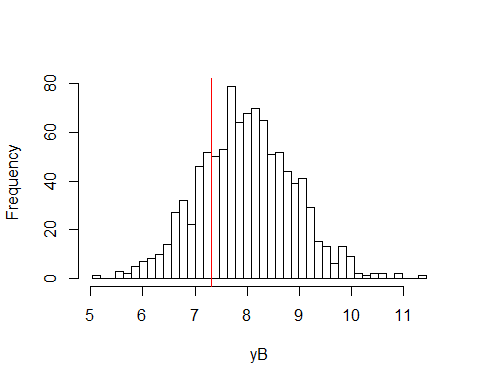
\includegraphics{STCI_files/figure-latex/histyb-1} 

}

\caption{Histogram of $y_B$}\label{fig:histyb}
\end{figure}

You can see on Figure \ref{fig:histyb} a histogram of \(y_i^B\) with the
red line indicating the cutoff point: \(\bar{y}=\ln(\bar{Y})=\) 7.3. All
the observations below the red line are treated according to the sharp
rule while all the one located above are not. In order to see how many
observations eventually receive the treatment with this allocation rule,
let's build a contingency table.

\begin{Shaded}
\begin{Highlighting}[]
\NormalTok{table.D.sharp <-}\StringTok{ }\KeywordTok{as.matrix}\NormalTok{(}\KeywordTok{table}\NormalTok{(Ds))}
\NormalTok{knitr}\OperatorTok{::}\KeywordTok{kable}\NormalTok{(table.D.sharp,}\DataTypeTok{caption=}\StringTok{'Treatment allocation with sharp cutoff rule'}\NormalTok{,}\DataTypeTok{booktabs=}\OtherTok{TRUE}\NormalTok{)}
\end{Highlighting}
\end{Shaded}

\begin{table}

\caption{\label{tab:tableDsharp}Treatment allocation with sharp cutoff rule}
\centering
\begin{tabular}[t]{lr}
\toprule
0 & 771\\
1 & 229\\
\bottomrule
\end{tabular}
\end{table}

We can see on Table \ref{tab:tableDsharp} that there are 229 treated
observations.

\subsubsection{The fuzzy cutoff rule}\label{the-fuzzy-cutoff-rule}

This rule is less sharp than the sharp cutoff rule. Here, other criteria
than \(Y_i^B\) enter into the decision to allocate the treatment. The
doctor might measure the health status of a patient following official
guidelines, but he might also measure other factors that will also
influence his decision of giving the drug to the patient. The officials
administering a program might measure the official income level of a
household, but they might also consider other features of the household
situation when deciding to enroll the household into the program or not.
If these additional criteria are unobserved to the econometrician, then
we have the fuzzy cutoff rule. A very simple way to model this rule is
as follows:

\begin{align}\label{eq:fuzzcutoff}
  D_i & = \uns{Y_i^B+V_i\leq\bar{Y}},
\end{align}

where \(V_i\) is a random variable unobserved to the econometrician and
standing for the other influences that might drive the allocation of the
treatment. \(V_i\) is distributed according to a, for the moment,
unspecified cumulative distribution function \(F_V\). When \(V_i\) is
degenerate (\textit{i.e.} it has only one point of support: it is a
constant), the fuzzy cutoff rule becomes the sharp cutoff rule.

\subsubsection{\texorpdfstring{The eligibility \(+\) self-selection
rule}{The eligibility + self-selection rule}}\label{the-eligibility-self-selection-rule}

It is also possible that households, once they have been made eligible
to the treatment, can decide whether they want to receive it or not. A
patient might be able to refuse the drug that the doctor suggests she
should take. A household might refuse to participate in a cash transfer
program to which it has been made eligible. Not all programs have this
feature, but most of them have some room for decisions by the agents
themselves of whether they want to receive the treatment or not. One
simple way to model this rule is as follows:

\begin{align}\label{eq:eligself}
  D_i & = \uns{D^*_i\geq0}E_i,
\end{align}

where \(D^*_i\) is individual \(i\)'s valuation of the treatment and
\(E_i\) is whether or not she is deemed eligible for the treatment.
\(E_i\) might be choosen according to the sharp cutoff rule of to the
fuzzy cutoff rule, or to any other eligibility rule. We will be more
explicit about \(D_i^*\) in what follows.

\textbf{SIMULATIONS ARE MISSING FOR THESE LAST TWO RULES}

\subsection{The potential outcomes}\label{the-potential-outcomes}

The second main building block of the RCM are potential outcomes. Let's
say that we are interested in the effect of a treatment on an outcome
\(Y\). Each unit \(i\) can thus be in two potential states: treated or
non treated. Before the allocation of the treatment is decided, both of
these states are feasible for each unit.

\BeginKnitrBlock{definition}[Potential outcomes]
\protect\hypertarget{def:unnamed-chunk-2}{}{\label{def:unnamed-chunk-2}
\iffalse (Potential outcomes) \fi{} }For each unit \(i\), we define two
potential outcomes:
\EndKnitrBlock{definition}

\begin{itemize}
\tightlist
\item
  \(Y_i^1\): the outcome that unit \(i\) is going to have if it receives
  the treatment,
\item
  \(Y_i^0\): the outcome that unit \(i\) is going to have if it
  \textbf{does not} receive the treatment.
\end{itemize}

\BeginKnitrBlock{example}
\protect\hypertarget{exm:unnamed-chunk-3}{}{\label{exm:unnamed-chunk-3}
}Let's choose functional forms for our potential outcomes. For
simplicity, all lower case letters will denote log outcomes.
\(y_i^0=\mu_i+\delta+U_i^0\), with \(\delta\) a time shock common to all
the observations and \(U_i^0=\rho U_i^B+\epsilon_i\), with \(|\rho|<1\).
In the absence of the treatment, part of the shocks \(U_i^B\) that the
individuals experienced in the previous period persist, while some part
vanish. \(y_i^1=y_i^0+\bar{\alpha}+\theta\mu_i+\eta_i\). In order to
generate the potential outcomes, one has to define the laws for the
shocks and to choose parameter values. Let's assume that
\(\epsilon_i\sim\mathcal{N}(0,\sigma^2_{\epsilon})\) and
\(\eta_i\sim\mathcal{N}(0,\sigma^2_{\eta})\). Now let's choose some
parameter values:
\EndKnitrBlock{example}

\begin{Shaded}
\begin{Highlighting}[]
\NormalTok{l <-}\StringTok{ }\KeywordTok{length}\NormalTok{(param)}
\NormalTok{param <-}\StringTok{ }\KeywordTok{c}\NormalTok{(param,}\FloatTok{0.9}\NormalTok{,}\FloatTok{0.01}\NormalTok{,}\FloatTok{0.05}\NormalTok{,}\FloatTok{0.05}\NormalTok{,}\FloatTok{0.05}\NormalTok{,}\FloatTok{0.1}\NormalTok{)}
\KeywordTok{names}\NormalTok{(param)[(l}\OperatorTok{+}\DecValTok{1}\NormalTok{)}\OperatorTok{:}\KeywordTok{length}\NormalTok{(param)] <-}\StringTok{ }\KeywordTok{c}\NormalTok{(}\StringTok{"rho"}\NormalTok{,}\StringTok{"theta"}\NormalTok{,}\StringTok{"sigma2epsilon"}\NormalTok{,}\StringTok{"sigma2eta"}\NormalTok{,}\StringTok{"delta"}\NormalTok{,}\StringTok{"baralpha"}\NormalTok{)}
\NormalTok{param}
\end{Highlighting}
\end{Shaded}

\begin{verbatim}
##         barmu      sigma2mu       sigma2U          barY           rho 
##          8.00          0.50          0.28       1500.00          0.90 
##         theta sigma2epsilon     sigma2eta         delta      baralpha 
##          0.01          0.05          0.05          0.05          0.10
\end{verbatim}

We can finally generate the potential outcomes;

\begin{Shaded}
\begin{Highlighting}[]
\NormalTok{epsilon <-}\StringTok{ }\KeywordTok{rnorm}\NormalTok{(N,}\DecValTok{0}\NormalTok{,}\KeywordTok{sqrt}\NormalTok{(param[}\StringTok{"sigma2epsilon"}\NormalTok{]))}
\NormalTok{eta<-}\StringTok{ }\KeywordTok{rnorm}\NormalTok{(N,}\DecValTok{0}\NormalTok{,}\KeywordTok{sqrt}\NormalTok{(param[}\StringTok{"sigma2eta"}\NormalTok{]))}
\NormalTok{U0 <-}\StringTok{ }\NormalTok{param[}\StringTok{"rho"}\NormalTok{]}\OperatorTok{*}\NormalTok{UB }\OperatorTok{+}\StringTok{ }\NormalTok{epsilon}
\NormalTok{y0 <-}\StringTok{ }\NormalTok{mu }\OperatorTok{+}\StringTok{  }\NormalTok{U0 }\OperatorTok{+}\StringTok{ }\NormalTok{param[}\StringTok{"delta"}\NormalTok{]}
\NormalTok{alpha <-}\StringTok{ }\NormalTok{param[}\StringTok{"baralpha"}\NormalTok{]}\OperatorTok{+}\StringTok{  }\NormalTok{param[}\StringTok{"theta"}\NormalTok{]}\OperatorTok{*}\NormalTok{mu }\OperatorTok{+}\StringTok{ }\NormalTok{eta}
\NormalTok{y1 <-}\StringTok{ }\NormalTok{y0}\OperatorTok{+}\NormalTok{alpha}
\NormalTok{Y0 <-}\StringTok{ }\KeywordTok{exp}\NormalTok{(y0)}
\NormalTok{Y1 <-}\StringTok{ }\KeywordTok{exp}\NormalTok{(y1)}
\end{Highlighting}
\end{Shaded}

Now, I would like to visualize my potential outcomes:

\begin{Shaded}
\begin{Highlighting}[]
\KeywordTok{plot}\NormalTok{(y0,y1)}
\end{Highlighting}
\end{Shaded}

\begin{figure}

{\centering 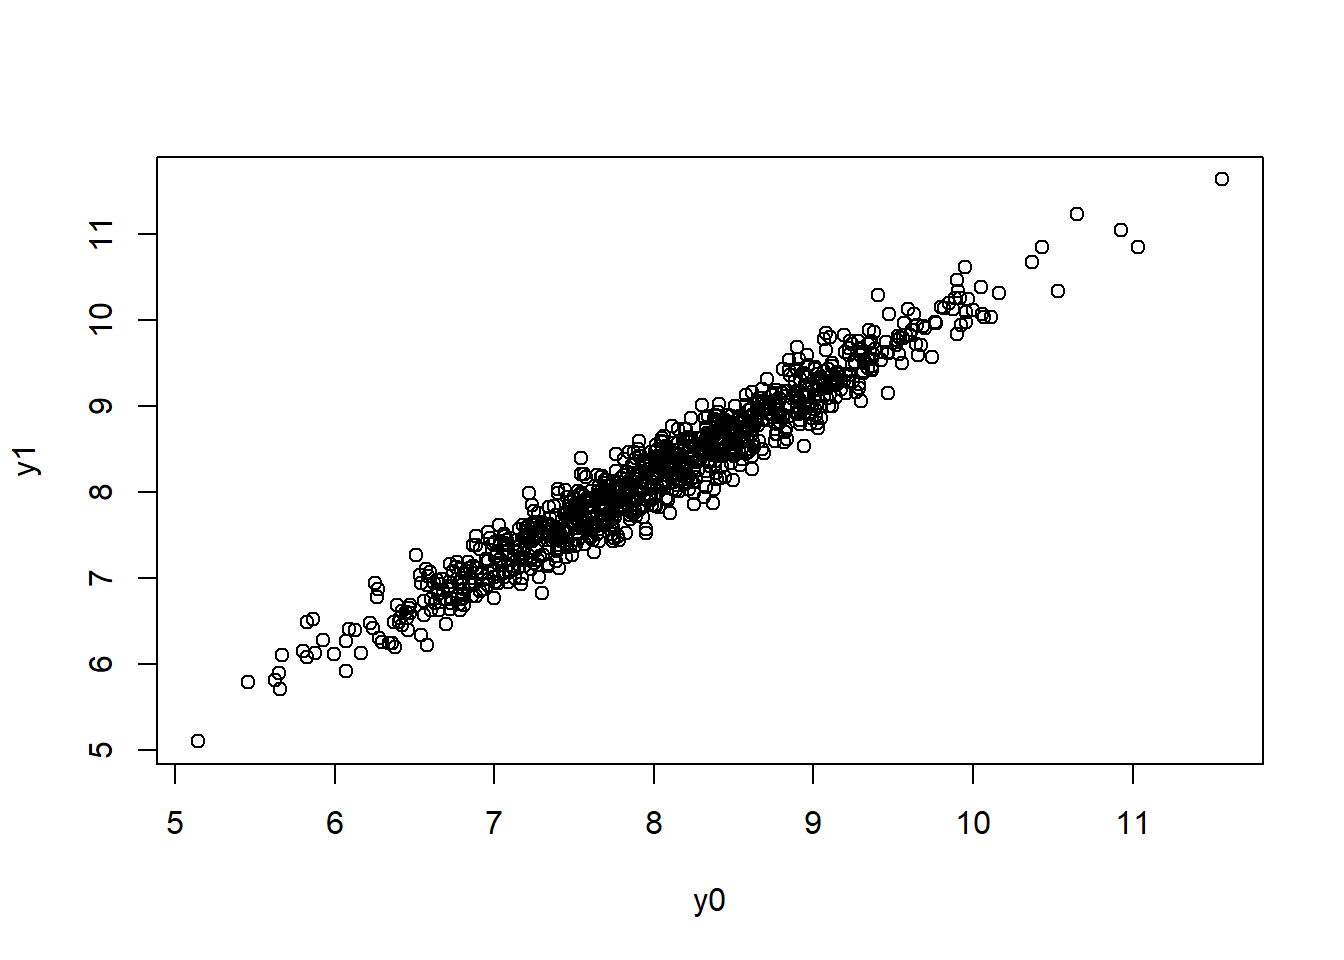
\includegraphics{STCI_files/figure-latex/histpotout-1} 

}

\caption{Potential outcomes}\label{fig:histpotout}
\end{figure}

You can see on the resulting Figure \ref{fig:histpotout} that both
potential outcomes are positively correlated. Those with a large
potential outcome when untreated (\emph{e.g.} in good health without the
treatment) also have a positive health with the treatment. It is also
true that individuals with bad health in the absence of the treatment
also have bad health with the treatment.

\subsection{The switching equation}\label{the-switching-equation}

The last building block of the RCM is the switching equation. It links
the observed outcome to the potential outcomes through the allocation
rule:

\begin{align}
 \label{eq:switch}
  Y_i & = 
    \begin{cases}
    Y_i^1 & \text{if } D_i=1\\
    Y_i^0 & \text{if } D_i=0
    \end{cases} \\
    & = Y_i^1D_i + Y_i^0(1-D_i) \nonumber
\end{align}

\BeginKnitrBlock{example}
\protect\hypertarget{exm:unnamed-chunk-4}{}{\label{exm:unnamed-chunk-4} }In
order to generate observed outcomes in our numerical example, we simply
have to enforce the switching equation:
\EndKnitrBlock{example}

\begin{Shaded}
\begin{Highlighting}[]
\NormalTok{y <-}\StringTok{ }\NormalTok{y1}\OperatorTok{*}\NormalTok{Ds}\OperatorTok{+}\NormalTok{y0}\OperatorTok{*}\NormalTok{(}\DecValTok{1}\OperatorTok{-}\NormalTok{Ds)}
\NormalTok{Y <-}\StringTok{ }\NormalTok{Y1}\OperatorTok{*}\NormalTok{Ds}\OperatorTok{+}\NormalTok{Y0}\OperatorTok{*}\NormalTok{(}\DecValTok{1}\OperatorTok{-}\NormalTok{Ds)}
\end{Highlighting}
\end{Shaded}

What the switching equation \eqref{eq:switch} means is that, for each
individual \(i\), we get to observe only one of the two potential
outcomes. When individual \(i\) belongs to the treatment group
(\emph{i.e.} \(D_i=1\)), we get to observe \(Y_i^1\). When individual
\(i\) belongs to the control group (\emph{i.e.} \(D_i=0\)), we get to
observe \(Y_i^0\). Because the same individual cannot be at the same
time in both groups, we can NEVER see both potential outcomes for the
same individual at the same time.

For each of the individuals, one of the two potential outcomes is
unobserved. We say that it is a \textbf{counterfactual}. A
counterfactual quantity is a quantity that is, according to Hume's
definition, contrary to the observed facts. A counterfactual cannot be
observed, but it can be conceived by an effort of reason: it is the
consequence of what would have happened had some action not been taken.

One very nice way of visualising the switching equation has been
proposed by Jerzy Neyman in a 1923 prescient paper. Neyman proposes to
imagine two urns, each one filled with \(N\) balls. One urn is the
treatment urn and contains balls with the id of the unit and the value
of its potential outcome \(Y_i^1\). The other urn is the control urn,
and it contains balls with the value of the potential outcome \(Y_i^0\)
for each unit \(i\). Following the allocation rule \(D_i\), we decide
whether unit \(i\) is in the treatment or control group. When unit \(i\)
is in the treatment group, we take the corresponding ball from the first
urn and observe the potential outcome on it. But, at the same time, the
urns are connected so that the corresponding ball with the potential
outcome of unit \(i\) in the control urn disappears as soon as we draw
ball \(i\) from the treatment urn.

The switching equation works a lot like Schrodinger's cat paradox.
Schrodinger's cat is placed in a sealed box and receives a dose of
poison when an atom emits a radiation. As long as the box is sealed,
there is no way we can know whether the cat is dead or alive. When we
open the box, we observe either a dead cat or a living cat, but we
cannot observe the cat both alice and dead at the same time. The
switching equation is like opening the box, it collapses the observed
outcome into one of the two potential ones.

\BeginKnitrBlock{example}
\protect\hypertarget{exm:unnamed-chunk-5}{}{\label{exm:unnamed-chunk-5} }One
way to visualize the inner workings of the switching equation is to plot
the potential outcomes along with the criteria driving the allocation
rule. In our simple example, it simply amounts to plotting observed
(\(y_i\)) and potential outcomes (\(y_i^1\) and \(y_i^0\)) along
\(y_i^B\).
\EndKnitrBlock{example}

\begin{Shaded}
\begin{Highlighting}[]
\KeywordTok{plot}\NormalTok{(yB[Ds}\OperatorTok{==}\DecValTok{0}\NormalTok{],y0[Ds}\OperatorTok{==}\DecValTok{0}\NormalTok{],}\DataTypeTok{pch=}\DecValTok{1}\NormalTok{,}\DataTypeTok{xlim=}\KeywordTok{c}\NormalTok{(}\DecValTok{5}\NormalTok{,}\DecValTok{11}\NormalTok{),}\DataTypeTok{ylim=}\KeywordTok{c}\NormalTok{(}\DecValTok{5}\NormalTok{,}\DecValTok{11}\NormalTok{),}\DataTypeTok{xlab=}\StringTok{"yB"}\NormalTok{,}\DataTypeTok{ylab=}\StringTok{"Outcomes"}\NormalTok{)}
\KeywordTok{points}\NormalTok{(yB[Ds}\OperatorTok{==}\DecValTok{1}\NormalTok{],y1[Ds}\OperatorTok{==}\DecValTok{1}\NormalTok{],}\DataTypeTok{pch=}\DecValTok{3}\NormalTok{)}
\KeywordTok{points}\NormalTok{(yB[Ds}\OperatorTok{==}\DecValTok{0}\NormalTok{],y1[Ds}\OperatorTok{==}\DecValTok{0}\NormalTok{],}\DataTypeTok{pch=}\DecValTok{3}\NormalTok{,}\DataTypeTok{col=}\StringTok{'red'}\NormalTok{)}
\KeywordTok{points}\NormalTok{(yB[Ds}\OperatorTok{==}\DecValTok{1}\NormalTok{],y0[Ds}\OperatorTok{==}\DecValTok{1}\NormalTok{],}\DataTypeTok{pch=}\DecValTok{1}\NormalTok{,}\DataTypeTok{col=}\StringTok{'red'}\NormalTok{)}
\NormalTok{test <-}\StringTok{ }\FloatTok{5.8}
\NormalTok{i.test <-}\StringTok{ }\KeywordTok{which}\NormalTok{(}\KeywordTok{abs}\NormalTok{(yB}\OperatorTok{-}\NormalTok{test)}\OperatorTok{==}\KeywordTok{min}\NormalTok{(}\KeywordTok{abs}\NormalTok{(yB}\OperatorTok{-}\NormalTok{test)))}
\KeywordTok{points}\NormalTok{(yB[}\KeywordTok{abs}\NormalTok{(yB}\OperatorTok{-}\NormalTok{test)}\OperatorTok{==}\KeywordTok{min}\NormalTok{(}\KeywordTok{abs}\NormalTok{(yB}\OperatorTok{-}\NormalTok{test))],y1[}\KeywordTok{abs}\NormalTok{(yB}\OperatorTok{-}\NormalTok{test)}\OperatorTok{==}\KeywordTok{min}\NormalTok{(}\KeywordTok{abs}\NormalTok{(yB}\OperatorTok{-}\NormalTok{test))],}\DataTypeTok{col=}\StringTok{'green'}\NormalTok{,}\DataTypeTok{pch=}\DecValTok{3}\NormalTok{)}
\KeywordTok{points}\NormalTok{(yB[}\KeywordTok{abs}\NormalTok{(yB}\OperatorTok{-}\NormalTok{test)}\OperatorTok{==}\KeywordTok{min}\NormalTok{(}\KeywordTok{abs}\NormalTok{(yB}\OperatorTok{-}\NormalTok{test))],y0[}\KeywordTok{abs}\NormalTok{(yB}\OperatorTok{-}\NormalTok{test)}\OperatorTok{==}\KeywordTok{min}\NormalTok{(}\KeywordTok{abs}\NormalTok{(yB}\OperatorTok{-}\NormalTok{test))],}\DataTypeTok{col=}\StringTok{'green'}\NormalTok{)}
\KeywordTok{abline}\NormalTok{(}\DataTypeTok{v=}\KeywordTok{log}\NormalTok{(param[}\StringTok{"barY"}\NormalTok{]),}\DataTypeTok{col=}\StringTok{"red"}\NormalTok{)}
\KeywordTok{legend}\NormalTok{(}\DecValTok{5}\NormalTok{,}\DecValTok{11}\NormalTok{,}\KeywordTok{c}\NormalTok{(}\StringTok{'y0|D=0'}\NormalTok{,}\StringTok{'y1|D=1'}\NormalTok{,}\StringTok{'y0|D=1'}\NormalTok{,}\StringTok{'y1|D=0'}\NormalTok{,}\KeywordTok{paste}\NormalTok{(}\StringTok{'y0'}\NormalTok{,i.test,}\DataTypeTok{sep=}\StringTok{''}\NormalTok{),}\KeywordTok{paste}\NormalTok{(}\StringTok{'y1'}\NormalTok{,i.test,}\DataTypeTok{sep=}\StringTok{''}\NormalTok{)),}\DataTypeTok{pch=}\KeywordTok{c}\NormalTok{(}\DecValTok{1}\NormalTok{,}\DecValTok{3}\NormalTok{,}\DecValTok{1}\NormalTok{,}\DecValTok{3}\NormalTok{,}\DecValTok{1}\NormalTok{,}\DecValTok{3}\NormalTok{),}\DataTypeTok{col=}\KeywordTok{c}\NormalTok{(}\StringTok{'black'}\NormalTok{,}\StringTok{'black'}\NormalTok{,}\StringTok{'red'}\NormalTok{,}\StringTok{'red'}\NormalTok{,}\StringTok{'green'}\NormalTok{,}\StringTok{'green'}\NormalTok{),}\DataTypeTok{ncol=}\DecValTok{3}\NormalTok{)}
\end{Highlighting}
\end{Shaded}

\begin{figure}

{\centering 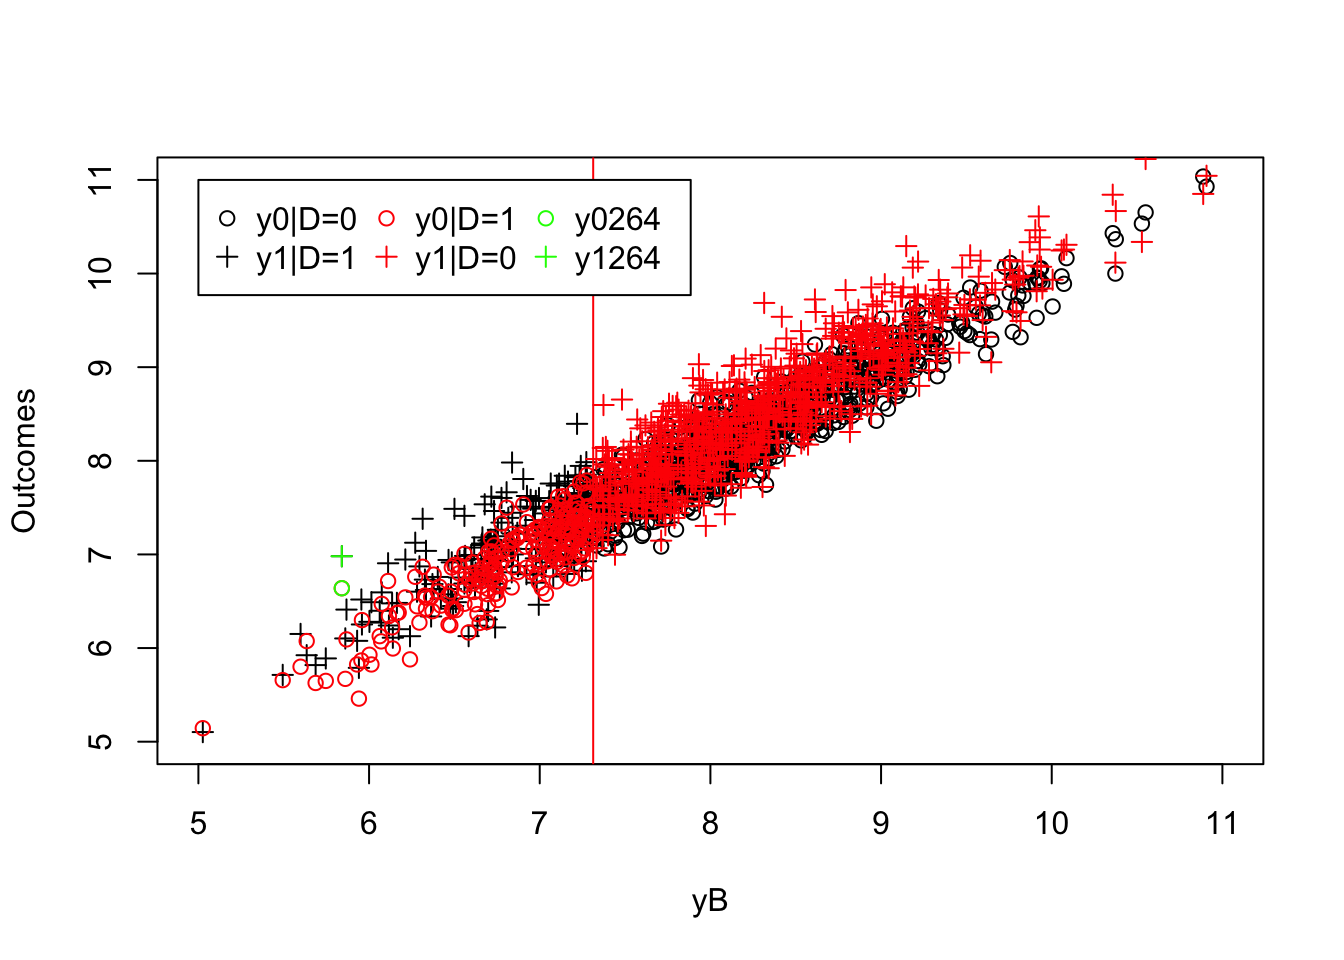
\includegraphics{STCI_files/figure-latex/plotyyB-1} 

}

\caption{Potential outcomes}\label{fig:plotyyB}
\end{figure}

\begin{Shaded}
\begin{Highlighting}[]
\KeywordTok{plot}\NormalTok{(yB[Ds}\OperatorTok{==}\DecValTok{0}\NormalTok{],y0[Ds}\OperatorTok{==}\DecValTok{0}\NormalTok{],}\DataTypeTok{pch=}\DecValTok{1}\NormalTok{,}\DataTypeTok{xlim=}\KeywordTok{c}\NormalTok{(}\DecValTok{5}\NormalTok{,}\DecValTok{11}\NormalTok{),}\DataTypeTok{ylim=}\KeywordTok{c}\NormalTok{(}\DecValTok{5}\NormalTok{,}\DecValTok{11}\NormalTok{),}\DataTypeTok{xlab=}\StringTok{"yB"}\NormalTok{,}\DataTypeTok{ylab=}\StringTok{"Outcomes"}\NormalTok{)}
\KeywordTok{points}\NormalTok{(yB[Ds}\OperatorTok{==}\DecValTok{1}\NormalTok{],y1[Ds}\OperatorTok{==}\DecValTok{1}\NormalTok{],}\DataTypeTok{pch=}\DecValTok{3}\NormalTok{)}
\KeywordTok{legend}\NormalTok{(}\DecValTok{5}\NormalTok{,}\DecValTok{11}\NormalTok{,}\KeywordTok{c}\NormalTok{(}\StringTok{'y|D=0'}\NormalTok{,}\StringTok{'y|D=1'}\NormalTok{),}\DataTypeTok{pch=}\KeywordTok{c}\NormalTok{(}\DecValTok{1}\NormalTok{,}\DecValTok{3}\NormalTok{))}
\KeywordTok{abline}\NormalTok{(}\DataTypeTok{v=}\KeywordTok{log}\NormalTok{(param[}\StringTok{"barY"}\NormalTok{]),}\DataTypeTok{col=}\StringTok{"red"}\NormalTok{)}
\end{Highlighting}
\end{Shaded}

\begin{figure}

{\centering 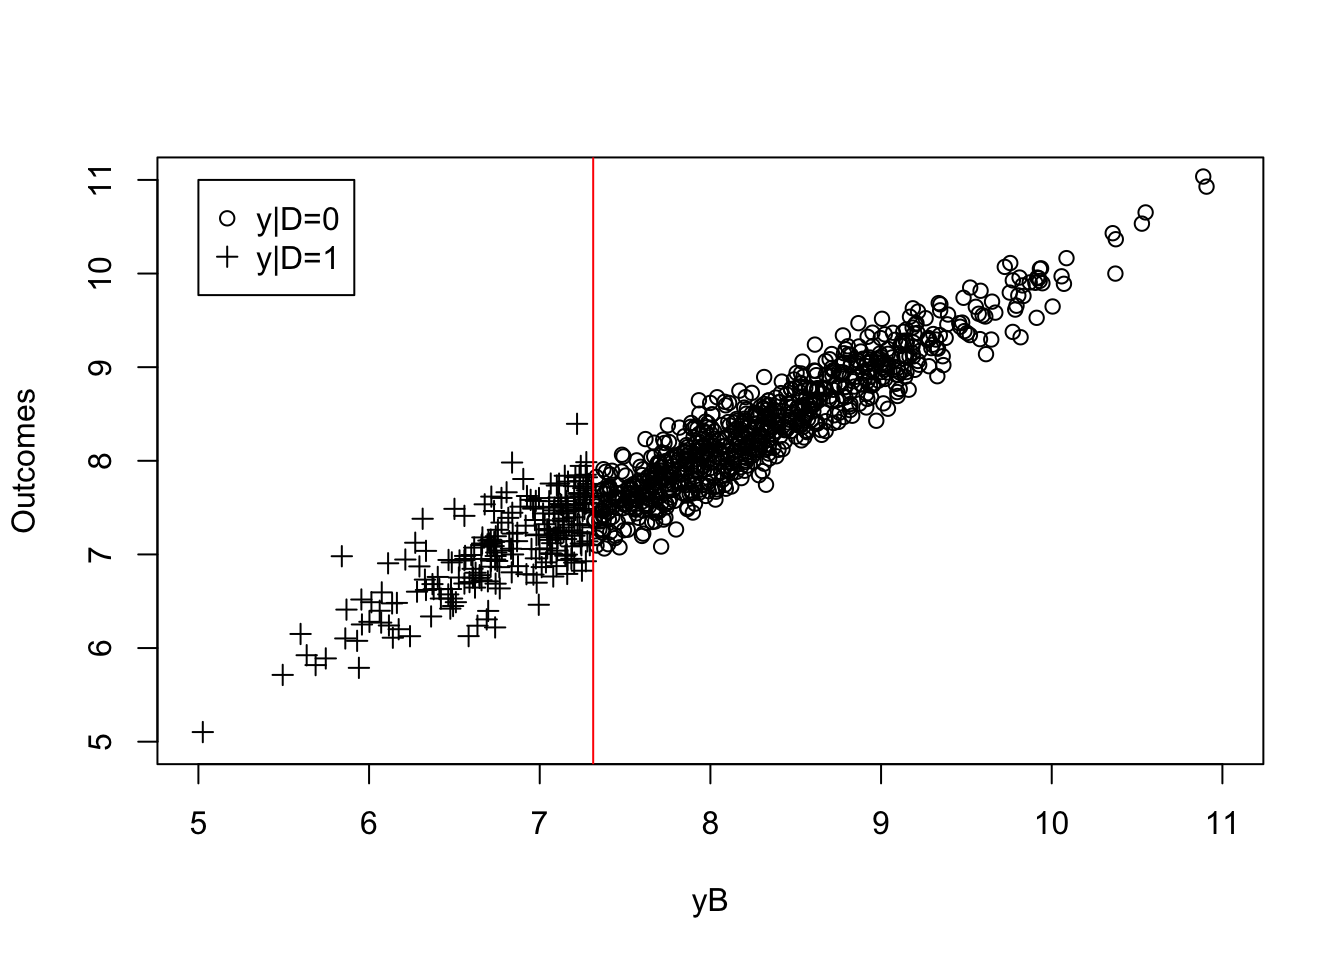
\includegraphics{STCI_files/figure-latex/ploty1y0yB-1} 

}

\caption{Observed outcomes}\label{fig:ploty1y0yB}
\end{figure}

Figure \ref{fig:ploty1y0yB} plots the observed outcomes \(y_i\) that
results from applying the switching equation. Figure
\ref{fig:ploty1y0yB} shows that each individual in the sample is endowed
with two potential outcomes, represented by a circle and a cross. Figure
\ref{fig:plotyyB} plots the observed outcomes \(y_i\) along with the
unobserved potential outcomes. Only one of the two potential outcomes is
observed (the cross for the treated group and the circle for the
untreated group) and the other is not. The observed sample in Figure
\ref{fig:plotyyB} only shows observed outcomes, and is thus silent on
the values of the missing potential outcomes.


\end{document}
